\documentclass[tikz,border=10pt]{standalone}
\usepackage{helvet}
\renewcommand{\familydefault}{\sfdefault}
\usetikzlibrary{positioning, arrows.meta, backgrounds, calc}

\begin{document}
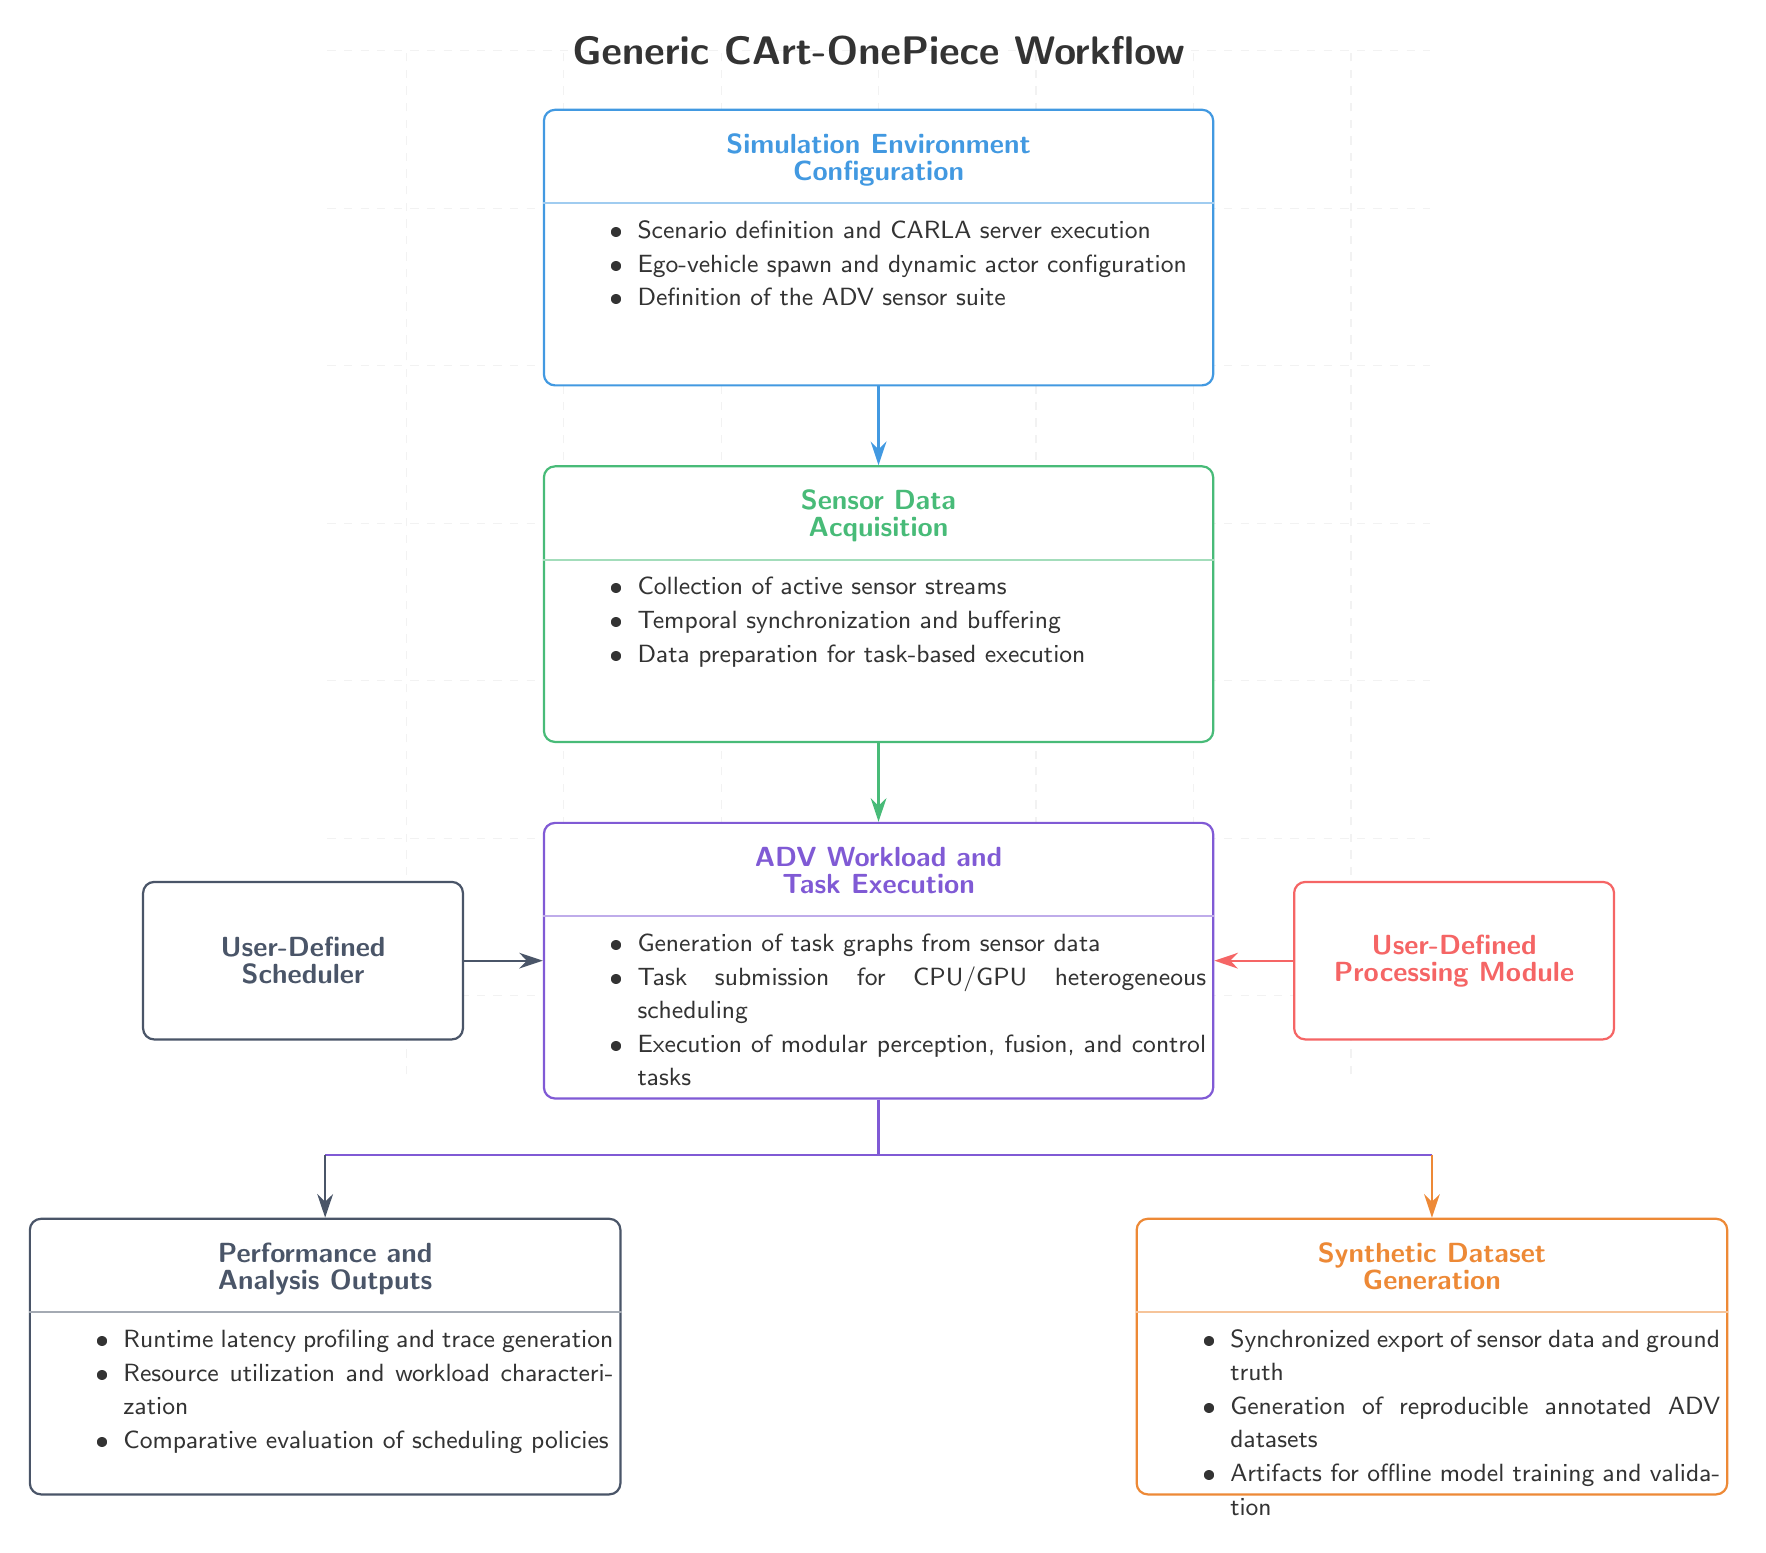
\begin{tikzpicture}[
    node distance=1cm and 0.5cm,
    >={Stealth[length=3mm, width=2mm]},
    box/.style={
        rectangle,
        draw=#1,
        fill=white,
        thick,
        rounded corners=4pt,
        align=left,
        text width=8.5cm,
        minimum height=3.5cm,
        inner sep=0pt
    },
    titlebox/.style={
        rectangle,
        draw=#1,
        fill=white,
        thick,
        rounded corners=4pt,
        align=center,
        text width=3.5cm,
        minimum height=2cm,
        font=\bfseries\color{#1},
        inner sep=8pt
    },
    arrow/.style={
        ->,
        thick,
        draw=#1
    },
    line/.style={
        thick,
        draw=#1
    }
]

% Colors
\definecolor{blue_color}{HTML}{4299E1}
\definecolor{green_color}{HTML}{48BB78}
\definecolor{purple_color}{HTML}{805AD5}
\definecolor{slate_color}{HTML}{4A5568}
\definecolor{red_color}{HTML}{F56565}
\definecolor{orange_color}{HTML}{ED8936}

% Grid Background (Optional for standalone, but adds the academic feel)
\begin{scope}[on background layer]
    \draw[black!5, dashed, step=2cm] (-7,-9) grid (7,4);
\end{scope}

% Title
\node[font=\Large\bfseries\color{black!80}, align=center, yshift=0.5cm] at (0, 3.5) {Generic CArt-OnePiece Workflow};

% Box 1
\node[box=blue_color] (B1) at (0,1.5) {};
\node[anchor=north, font=\bfseries\color{blue_color}, align=center, yshift=-0.2cm] at (B1.north) {Simulation Environment\\[-0.5ex]Configuration};
\draw[blue_color!50, thick] ([yshift=-1.2cm]B1.north west) -- ([yshift=-1.2cm]B1.north east);
\node[anchor=north west, font=\small\linespread{1.1}\selectfont\color{black!80}, align=left, yshift=-1.3cm, xshift=0.2cm] at (B1.north west) {
    \begin{minipage}{8.1cm}
    \begin{itemize}\setlength\itemsep{-0.2em}
        \item Scenario definition and CARLA server execution
        \item Ego-vehicle spawn and dynamic actor configuration
        \item Definition of the ADV sensor suite
    \end{itemize}
    \end{minipage}
};

% Box 2
\node[box=green_color, below=of B1] (B2) {};
\node[anchor=north, font=\bfseries\color{green_color}, align=center, yshift=-0.2cm] at (B2.north) {Sensor Data\\[-0.5ex]Acquisition};
\draw[green_color!50, thick] ([yshift=-1.2cm]B2.north west) -- ([yshift=-1.2cm]B2.north east);
\node[anchor=north west, font=\small\linespread{1.1}\selectfont\color{black!80}, align=left, yshift=-1.3cm, xshift=0.2cm] at (B2.north west) {
    \begin{minipage}{8.1cm}
    \begin{itemize}\setlength\itemsep{-0.2em}
        \item Collection of active sensor streams
        \item Temporal synchronization and buffering
        \item Data preparation for task-based execution
    \end{itemize}
    \end{minipage}
};

% Box 3
\node[box=purple_color, below=of B2] (B3) {};
\node[anchor=north, font=\bfseries\color{purple_color}, align=center, yshift=-0.2cm] at (B3.north) {ADV Workload and\\[-0.5ex]Task Execution};
\draw[purple_color!50, thick] ([yshift=-1.2cm]B3.north west) -- ([yshift=-1.2cm]B3.north east);
\node[anchor=north west, font=\small\linespread{1.1}\selectfont\color{black!80}, align=left, yshift=-1.3cm, xshift=0.2cm] at (B3.north west) {
    \begin{minipage}{8.1cm}
    \begin{itemize}\setlength\itemsep{-0.2em}
        \item Generation of task graphs from sensor data
        \item Task submission for CPU/GPU heterogeneous scheduling
        \item Execution of modular perception, fusion, and control tasks
    \end{itemize}
    \end{minipage}
};

% Side Box 1 (Left)
\node[titlebox=slate_color, left=of B3, xshift=-0.5cm] (S1) {User-Defined\\[-0.5ex]Scheduler};

% Side Box 2 (Right)
\node[titlebox=red_color, right=of B3, xshift=0.5cm] (S2) {User-Defined\\[-0.5ex]Processing Module};

% Box 4
\node[box=slate_color, below left=of B3, text width=7.5cm, xshift=1.5cm, yshift=-0.5cm] (B4) {};
\node[anchor=north, font=\bfseries\color{slate_color}, align=center, yshift=-0.2cm] at (B4.north) {Performance and\\[-0.5ex]Analysis Outputs};
\draw[slate_color!50, thick] ([yshift=-1.2cm]B4.north west) -- ([yshift=-1.2cm]B4.north east);
\node[anchor=north west, font=\small\linespread{1.1}\selectfont\color{black!80}, align=left, yshift=-1.3cm, xshift=0.2cm] at (B4.north west) {
    \begin{minipage}{7.1cm}
    \begin{itemize}\setlength\itemsep{-0.2em}
        \item Runtime latency profiling and trace generation
        \item Resource utilization and workload characterization
        \item Comparative evaluation of scheduling policies
    \end{itemize}
    \end{minipage}
};

% Box 5
\node[box=orange_color, below right=of B3, text width=7.5cm, xshift=-1.5cm, yshift=-0.5cm] (B5) {};
\node[anchor=north, font=\bfseries\color{orange_color}, align=center, yshift=-0.2cm] at (B5.north) {Synthetic Dataset\\[-0.5ex]Generation};
\draw[orange_color!50, thick] ([yshift=-1.2cm]B5.north west) -- ([yshift=-1.2cm]B5.north east);
\node[anchor=north west, font=\small\linespread{1.1}\selectfont\color{black!80}, align=left, yshift=-1.3cm, xshift=0.2cm] at (B5.north west) {
    \begin{minipage}{7.1cm}
    \begin{itemize}\setlength\itemsep{-0.2em}
        \item Synchronized export of sensor data and ground truth
        \item Generation of reproducible annotated ADV datasets
        \item Artifacts for offline model training and validation
    \end{itemize}
    \end{minipage}
};

% Arrows
\draw[arrow=blue_color] (B1.south) -- (B2.north);
\draw[arrow=green_color] (B2.south) -- (B3.north);

\draw[arrow=slate_color] (S1.east) -- (B3.west);
\draw[arrow=red_color] (S2.west) -- (B3.east);

% Branching Arrows
\coordinate (split) at ($(B3.south) + (0, -0.7cm)$);
\draw[line=purple_color] (B3.south) -- (split);
\draw[line=purple_color] (B4.north |- split) -- (B5.north |- split);
\draw[arrow=slate_color] (B4.north |- split) -- (B4.north);
\draw[arrow=orange_color] (B5.north |- split) -- (B5.north);

\end{tikzpicture}
\end{document}
